\documentclass[12pt]{article}
\usepackage{zh_CN-Adobefonts_external} % Simplified Chinese Support using external fonts (./fonts/zh_CN-Adobe/)
% fonts
\usepackage[scaled=0.92]{helvet}   % set Helvetica as the sans-serif font
\renewcommand{\rmdefault}{ptm}     % set Times as the default text font

% dmb: not mandatory, but i recommend you use mtpro for math fonts.
% there is a free version called mtprolite.

% \usepackage[amssymbols,subscriptcorrection,slantedGreek,nofontinfo]{mtpro2}

\usepackage[T1]{fontenc}
\usepackage{amsmath}
\usepackage{amsfonts}

% page numbers
\usepackage{fancyhdr}
\fancypagestyle{newstyle}{
\fancyhf{} % clear all header and footer fields
\fancyfoot[R]{\vspace{0.1in} \small \thepage}
\renewcommand{\headrulewidth}{0pt}
\renewcommand{\footrulewidth}{0pt}}
\pagestyle{newstyle}

% geometry of the page
\usepackage[top=1in, bottom=1in, left=1.625in, right=1.625in]{geometry}

% paragraph spacing
\setlength{\parindent}{0pt}
\setlength{\parskip}{2ex plus 0.4ex minus 0.2ex}

% useful packages
\usepackage{natbib}
\usepackage{epsfig}
\usepackage{url}
\usepackage{bm}


\begin{document}

\begin{center}
  \Large \textbf{XXX协作计算平台用户指南} \\
  \vspace{0.1in}
  \normalsize 国际应用数据科学研究院 \\
  \today
\end{center}

\tableofcontents
\newpage

\section {XXX协作计算平台简介}


\section {使用指南}
在使用本指南之前,用户需要向所在单位网络运营管理部门申请IP地址和域名,为后续运营管理该协作计算平台做好准备工作。
\subsection{登陆管理平台}
打开浏览器,输入协作管理平台IP地址XXX.XXX.XXX.XXX或域名www.xxx.xxx.com,回车,得到如图\ref{fig:login}所示登陆界面。

\begin{figure}[!htb]
\centering
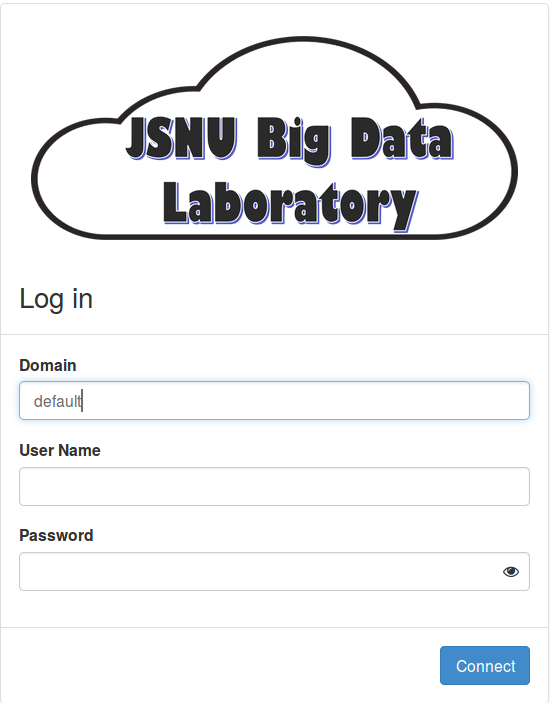
\includegraphics[width=6in]{./figures/login}
%\includegraphics[height=2.1338in, width=3.3307in]{./the_directed_neighbor_tree.png}
%\epsfig{file=./Fig1.png,height=2.1338in, width=3.3307in}
\caption{登陆界面}
\label{fig:login}
\end{figure}
在该页面需要用户输入域名(\textbf{domain})、用户名(\textbf{user name})以及密码(\textbf{password})。这里域名跟上面提到域名不同,用户只需要输入\textbf{default}即可,用户名和密码则为协作平台管理员为不同用户分配的用户名和密码。输入完毕,点击\textbf{Sign In},进入协作平台管理界面如图\ref{fig:afterLogin}。如果以普通用户身份登陆系统,该页面只显示项目选项(\textbf{Project});如果以管理员身份登陆,该页面显示项目选项(\textbf{Project})、管理选项(\textbf{Admin})以及标识选项(\textbf{Identyty})。
\begin{figure}[!htb]
\centering
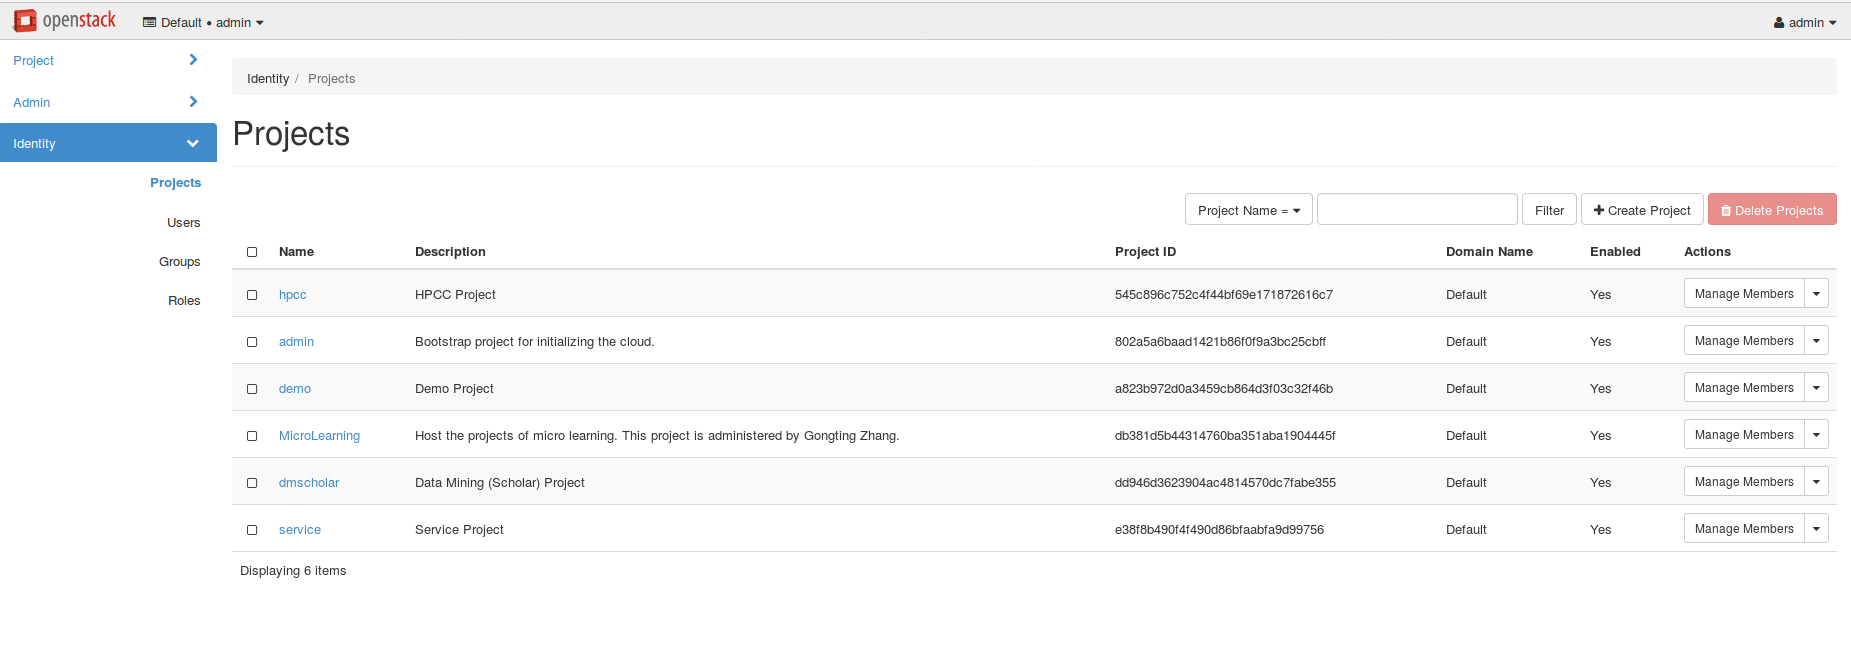
\includegraphics[width=6in]{./figures/afterLogin}
%\includegraphics[height=2.1338in, width=3.3307in]{./the_directed_neighbor_tree.png}
%\epsfig{file=./Fig1.png,height=2.1338in, width=3.3307in}
\caption{协作平台管理界面}
\label{fig:afterLogin}
\end{figure}
\subsubsection{项目信息}
该协作平台以项目为组织单位进行管理,用户可以同时参与多个项目,并在项目中创建、管理计算资源。

点击项目选项(\textbf{Project}),用户可以查看、管理每个项目的计算资源如图\ref{fig:projectOverview}
\begin{figure}[!htb]
\centering
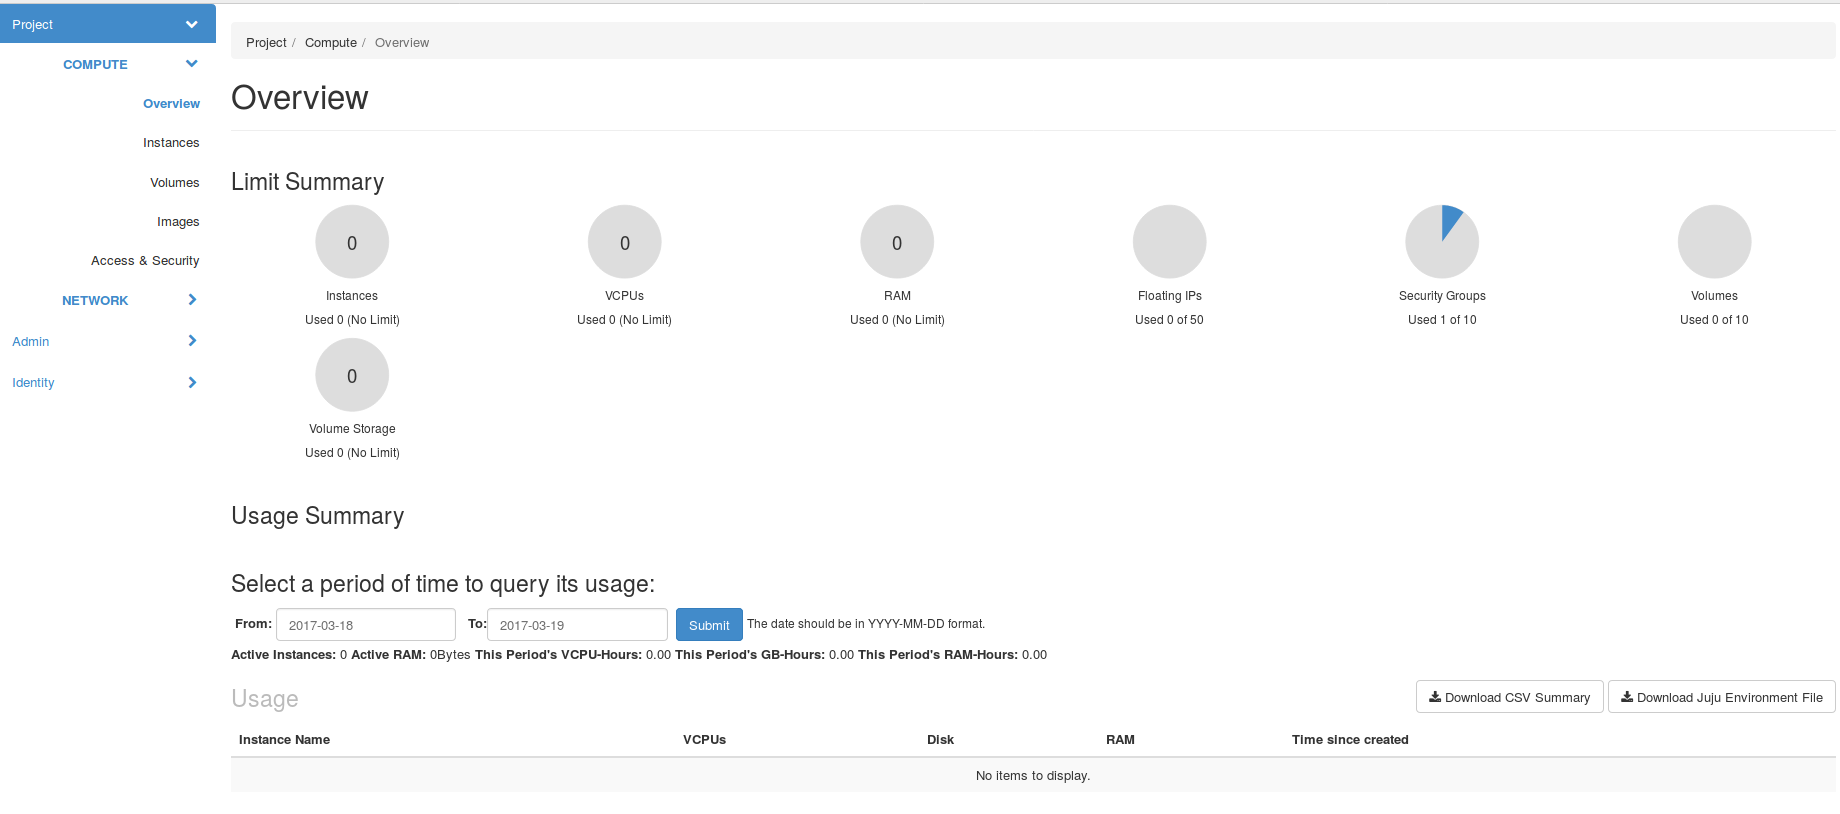
\includegraphics[width=6in]{./figures/projectOverview}
%\includegraphics[height=2.1338in, width=3.3307in]{./the_directed_neighbor_tree.png}
%\epsfig{file=./Fig1.png,height=2.1338in, width=3.3307in}
\caption{项目选项}
\label{fig:projectOverview}
\end{figure}
从项目选项,用户可以访问如表\ref{tab:project}所示子选项。
\begin{table}[!htb]
\centering
\caption{通过项目选项可访问的子选项}  \label{tab:project}
\begin{tabular}{c|p{8cm}} \hline
计算选项\textbf{Compute Tab} & \\ \hline
\textbf{Overview}& 查看项目报告\\ \hline
\textbf{Instances} & 查看、启动、创建快照,停止、暂停、重启实例,也可以通过VNC连接这些实例\\ \hline
Volumes & 该子选项下又包括两个子选项,其中通过Volumes子选项可以查看、创建、编辑、删除volumes;通过Volume Snapshots子选项可以查看、创建、编辑、删除volume快照。 \\ \hline
\textbf{Images} & 查看项目用户创建的镜像和实例快照,创建、编辑以及删除镜像,从镜像或快照启动实例。 \\ \hline
\textbf{Access \& Security} & 为实例创建安全访问策略,其中\textbf{Security Groups}查看、创建、编辑以及删除安全组和相应规则;\textbf{Key Pairs}查看、创建、编辑、导入以及删除健对;\textbf{Floating IPs}为项目分配IP地址 \\ \hline
\textbf{Network tab} &  \\ \hline
\textbf{Network Topology} & 查看网络拓扑 \\ \hline
\textbf{Compute tab} &  \\ \hline
\textit{Networks} & 创建、管理公共、私有网络 \\ \hline
\textit{Routers} & 创建、管理子网 \\
\textit{Object Store tab}& \\ \hline
\textit{Containers} & 创建、管理容器和对象 \\ \hline
\textit{Orchestration tab} &  \\
\textit{Stacks}& 通过\textit{REST API}组织多个复合云应用 \\ \hline
\end{tabular}
\end{table}
\subsubsection{\textbf{Admin}选项}
管理员通过\textbf{Admin}选项查看、管理实例,Volumes, flavors, images, projects, users, services, and quotas。
\begin{figure}[!htb]
\centering
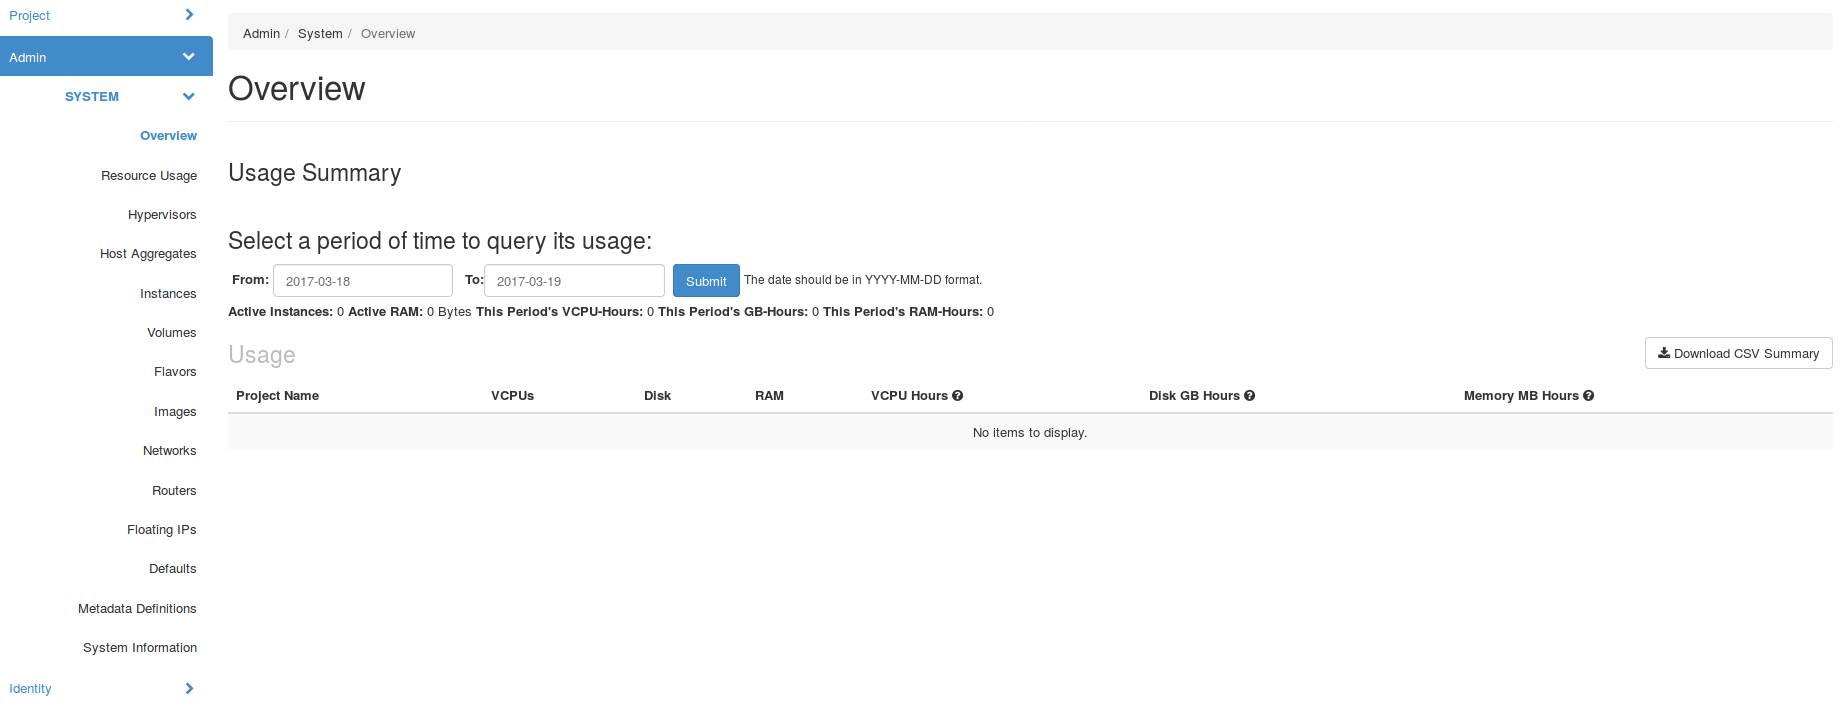
\includegraphics[width=6in]{./figures/adminOverview}
%\includegraphics[height=2.1338in, width=3.3307in]{./the_directed_neighbor_tree.png}
%\epsfig{file=./Fig1.png,height=2.1338in, width=3.3307in}
\caption{Admin选项}
\label{fig:adminOverview}
\end{figure}
通过\textbf{Admin}选项可以完成如表\ref{tab:admin}任务。
\begin{table}[!htb]
\centering
\caption{通过项目选项可访问的子选项}  \label{tab:admin}
\begin{tabular}{c|p{8cm}} \hline
\textbf{Overview}& 查看报告\\ \hline
\textbf{Resource Usage} & \textbf{Daily Report}查看日报表,\textbf{Stats}查看所有资源使用统计数据\\ \hline
\textbf{Hypervisors} & 查看虚拟机监视器汇总信息\\ \hline
\textbf{Host Aggregates} & 查看、创建、编辑host aggregates,查看可用域 \\ \hline
\textbf{Instances} & 查看、停止、暂停、重启、挂起、迁移、删除运行一些项目实例,查看实例运行日志或者通过VNC访问实例。 \\ \hline
\textbf{Volumes} & 查看、创建、编辑、删除volumes and volume type\\ \hline
\textbf{Flavors} & 查看、创建、编辑、删除flavors. a flavor is size of an instance \\ \hline
\textbf{Images} & 查看、创建、编辑、删除定制镜像 \\ \hline
\textit{Networks} & 查看、创建、编辑、删除网络 \\ \hline
\textit{Routers} & 查看、创建、编辑、删除路由器 \\

\textit{System Info}& \textbf{Services}查看服务列表,\textbf{Compute Services}查看所有计算服务,\textbf{Network Agents}查看网络代理,\textbf{Default Quotas}查看默认配额\\ \hline
\textit{Identity} &  \\ \hline
\textit{Projects} & 查看、创建、用户分配、去除用户以及删除项目 \\
\textit{Users}& 查看、创建、激活、注销、删除用户 \\ \hline
\end{tabular}
\end{table}
\subsection{管理项目和用户}
本小节概要:如何添加、更新、删除项目和用户;如何分配用户至多个项目,以及如何修改或移除用户分配;如何激活或暂时注销项目或用户。

\subsubsection{创建项目}
1. 登陆协作管理平台界面,从左侧管理列表选择``Identity''->``project'',进入如图\ref{fig:createProject}页面,在该页面右上侧点击``+Create Project'',弹出如图\ref{fig:createProject_1}所示窗口,在``Project Information''中输入项目名称和相应描述信息,另外2项``Domain ID''、``Domain Name''不做修改;点击该窗口``Project Members'',添加用户至该新建项目,或者通过点击``Project Groups''为该新建项目批量添加用户;点击``Quota'',编辑该新建项目所需计算、存储、网络等资源配额;最后点击右下角``Create Project'',完成项目创建。
\begin{figure}[!htb]
\centering
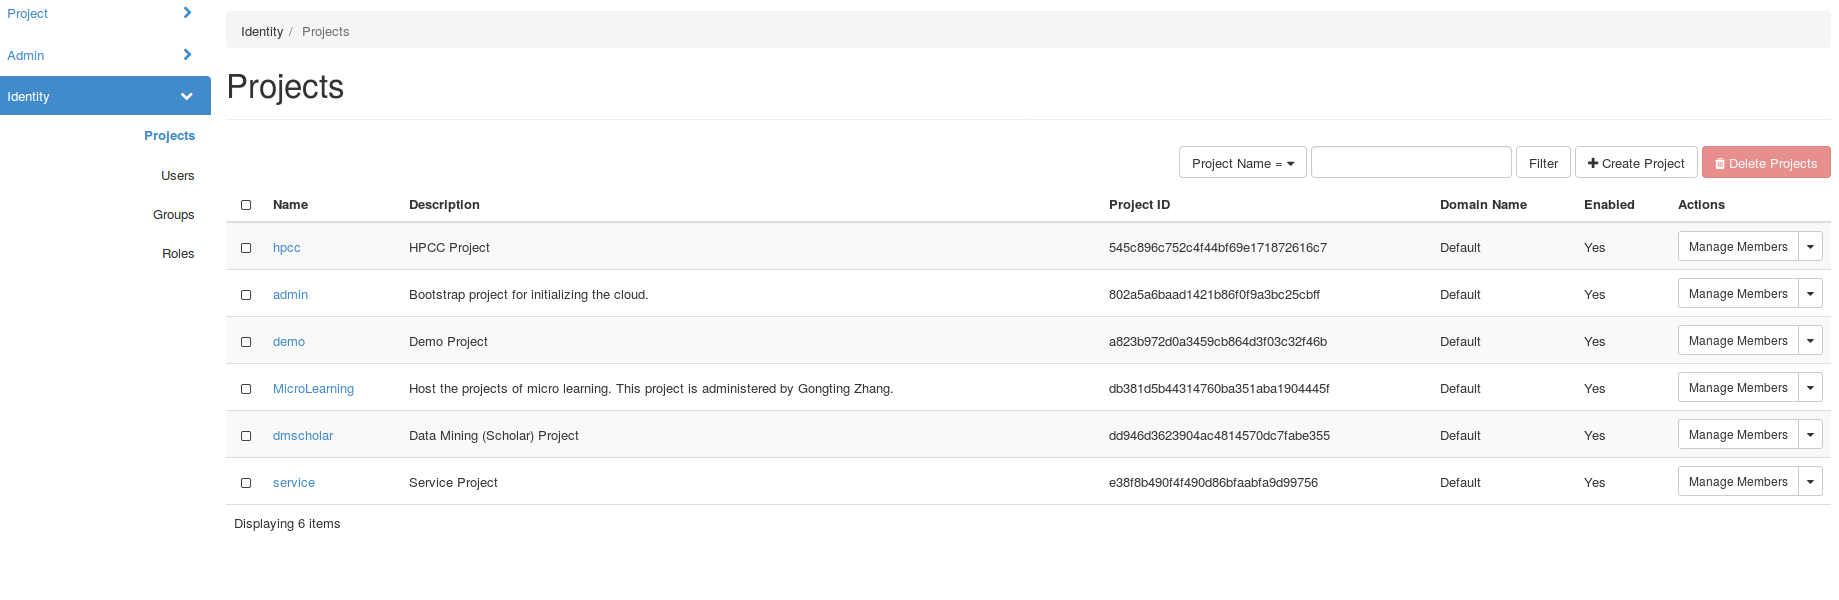
\includegraphics[width=6in]{./figures/createProject}
%\includegraphics[height=2.1338in, width=3.3307in]{./the_directed_neighbor_tree.png}
%\epsfig{file=./Fig1.png,height=2.1338in, width=3.3307in}
\caption{创建项目}
\label{fig:createProject}
\end{figure}
\begin{figure}[!htb]
\centering
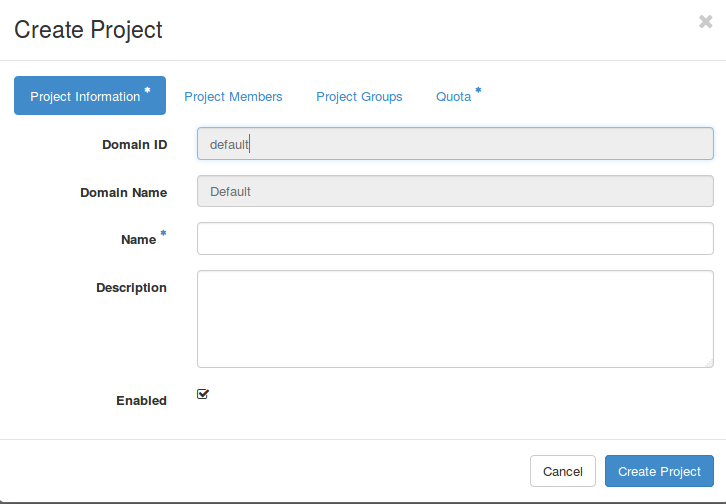
\includegraphics[width=6in]{./figures/createProject_1}
%\includegraphics[height=2.1338in, width=3.3307in]{./the_directed_neighbor_tree.png}
%\epsfig{file=./Fig1.png,height=2.1338in, width=3.3307in}
\caption{创建项目}
\label{fig:createProject_1}
\end{figure}
\subsubsection{更新项目}
项目创建完成后,用户还可以对项目进行如修改项目名称和描述、激活、暂时注销等更新动作。
1. 在管理选项(\textbf{Admin})中,打开\textbf{Identity}面板,点击\textbf{``Projects''},然后选择拟更新项目;
2. 在\textbf{``More''}下拉菜单中点击\textbf{``Edit Project''},在弹出窗口完成对项目的更新;
3. 点击\textbf{``Save''}进行保存。
\textbf{备注:}
$\bullet$ 被注销的项目将不在\textbf{``CURRENT PROJECT''}下拉菜单中显示;\\
$\bullet$ 唯一隶属于被注销项目的用户将不能再登陆;\\
$\bullet$ 被注销项目数据仍然被系统保存,管理员可以重新启用被注销项目;
\subsubsection{修改项目用户成员}
管理员可以动态为项目添加、删除用户成员。\\
$\bullet$ 进入管理界面,点击\textbf{``Identity''}->\textbf{``Projects''},点击拟修改项目或在拟修改项目行最右侧下拉菜单中选择\textbf{``Edit Project''},在弹出如图\ref{fig:editProject}页面进行修改。
\begin{figure}[!htb]
\centering
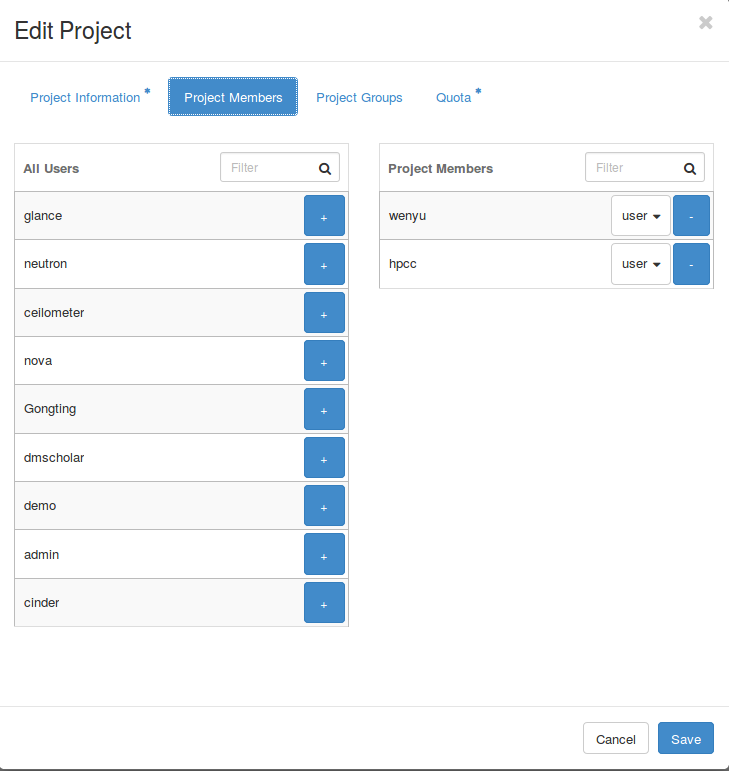
\includegraphics[width=6in]{./figures/editProject}
\caption{修改项目成员}
\label{fig:editProject}
\end{figure}
左侧\textbf{``All Users''}列显示所有可选用户,右侧\textbf{``Project Members''}显示已分配到该项目的用户;点击左侧对应用户\textbf{``+''},将该用户添加至该项目;在右侧\textbf{``Project Members''}列,点击相应用户\textbf{``-''},将该用户移出该项目;最后点击\textbf{``Save''}保存。
\subsubsection{删除项目}
删除项目操作如图\ref{fig:deleteProject}。在\textbf{``Identity‘’}下拉菜单中点击\textbf{``Projects''},在对应项目行最右侧下拉菜单中选择\textbf{``Delete Project''},完成项目删除。
\begin{figure}[!htb]
\centering
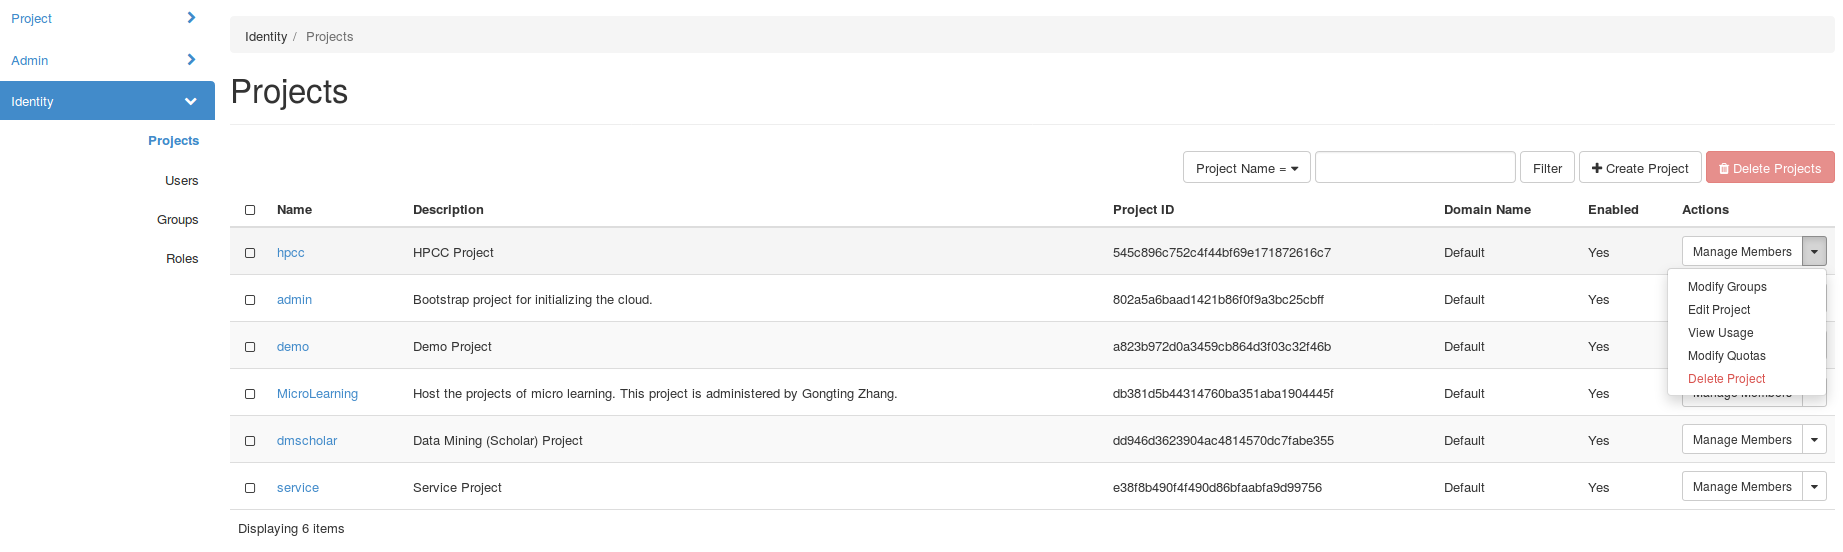
\includegraphics[width=6in]{./figures/deleteProject}
\caption{删除项目}
\label{fig:deleteProject}
\end{figure}
\textbf{备注:}项目一旦被删除,将不能被恢复。
\subsubsection{创建用户}
管理员通过如图\ref{fig:createUser}、图\ref{fig:createUser1}界面创建用户帐号。首先点击\textbf{``Identity''}下拉列表,选择\textbf{``Users''},在弹出页面点击\textbf{``+Create User''}按钮并显示如图\ref{fig:createUser1}所示页面,输入用户相关信息,最后点击右下角\textbf{``Create User''}按钮完成创建。
\begin{figure}[!htb]
\centering
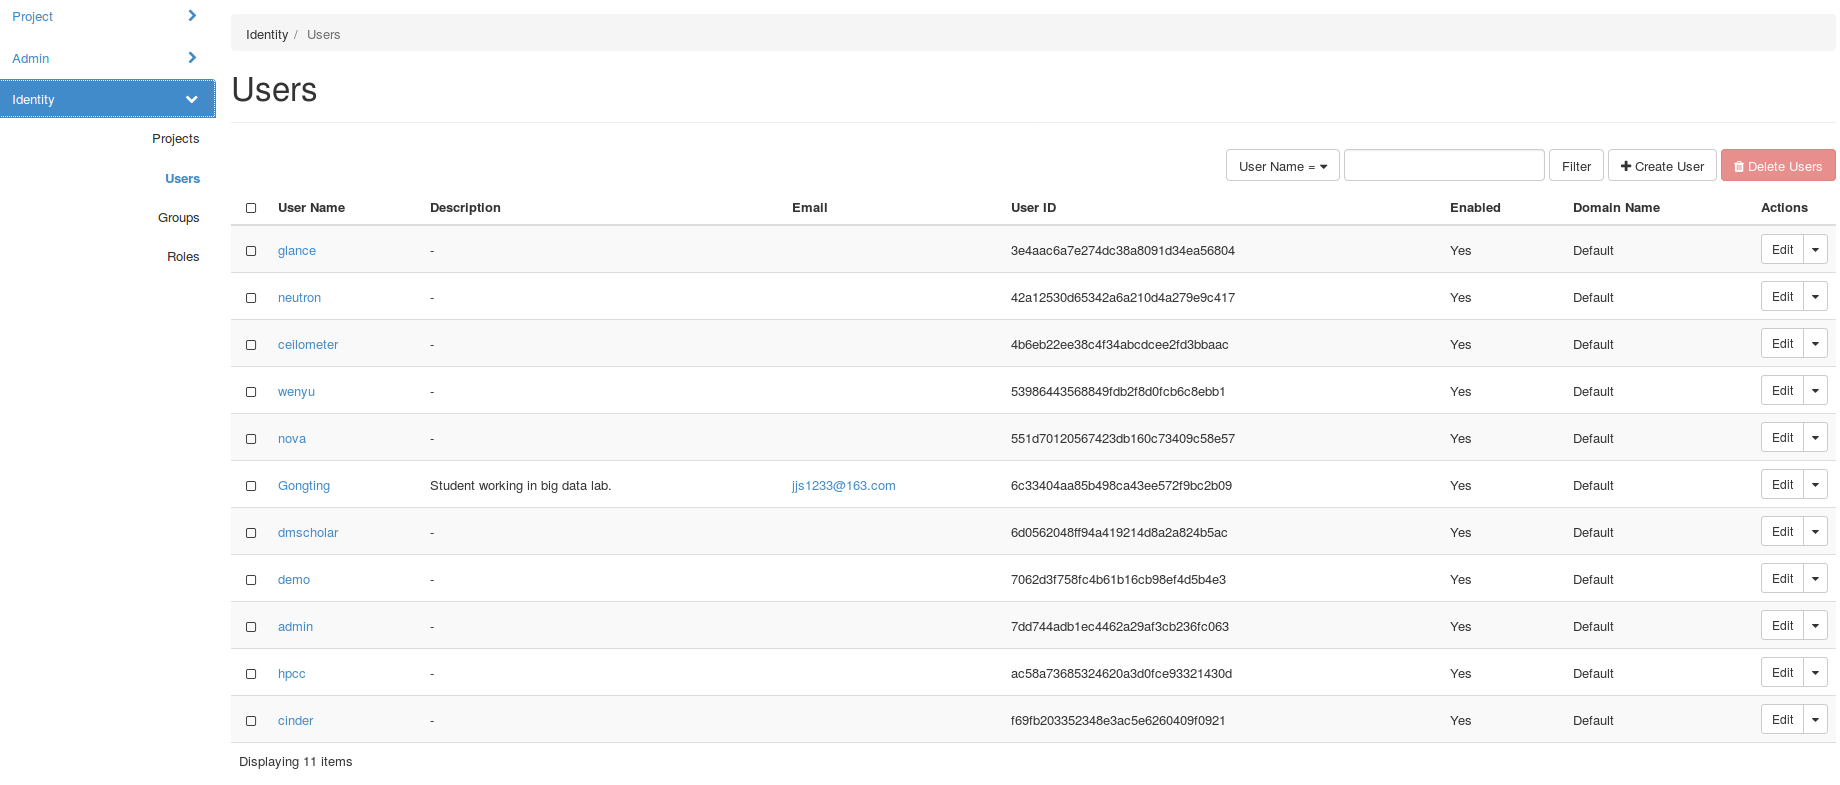
\includegraphics[width=6in]{./figures/createUser}
\caption{创建用户}
\label{fig:createUser}
\end{figure}
\begin{figure}[!htb]
\centering
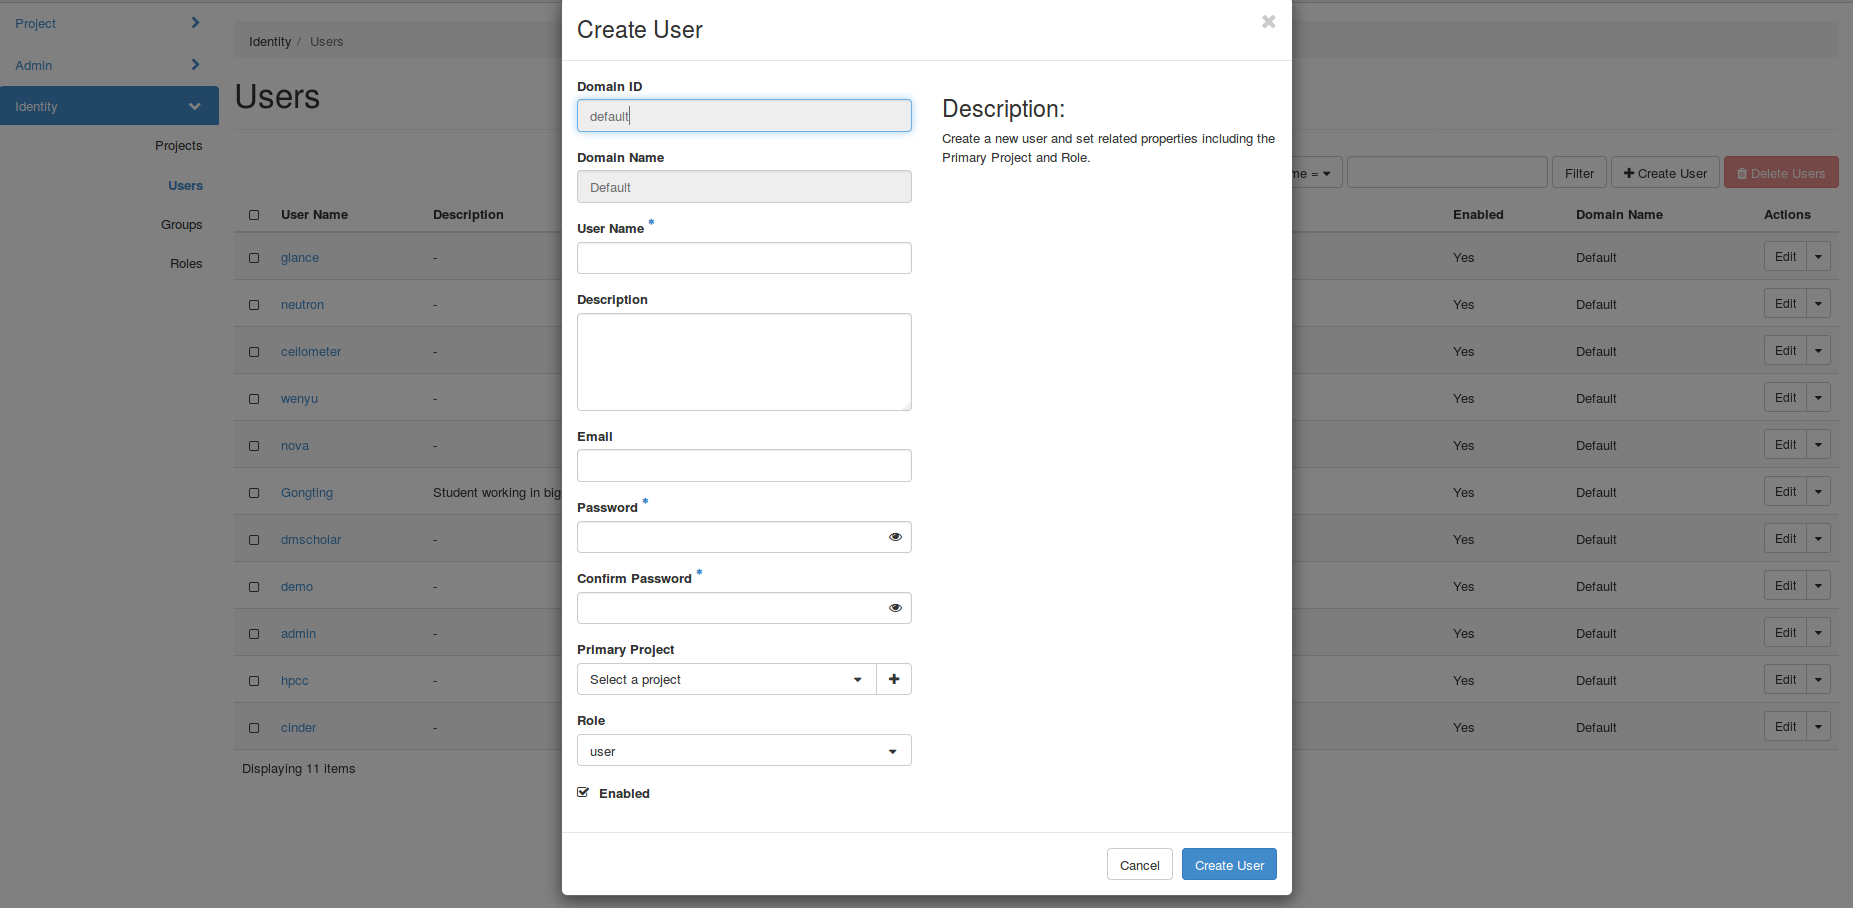
\includegraphics[width=6in]{./figures/createUser1}
\caption{创建用户}
\label{fig:createUser1}
\end{figure}

\subsection{镜像制作}
\subsubsection{镜像源下载}
镜像是虚拟机操作系统的源,本协作计算平台支持linux、windows等多种操作系统。在制作镜像之前,用户需要下载相应镜像软件包至本地。下面首先给出几种常用操作系统镜像下载地址(具体请参考https://docs.openstack.org/image-guide/obtain-images.html):
Centor 6 镜像 http://cloud.centos.org/centos/6/images/ \\
Centor 7 镜像 http://cloud.centos.org/centos/7/images/ \\
CirrOS 镜像 http://download.cirros-cloud.net/ \\
Debian 镜像 http://cdimage.debian.org/cdimage/openstack/ \\
Fedora 镜像 https://getfedora.org/cloud/download/ \\
Ubuntu 镜像 http://cloud-images.ubuntu.com/
\subsubsection{镜像制作流程}
在协作平台管理界面,点击``\textbf{Project}''->``\textbf{Compute}''->``\textbf{Images}''进入如图\ref{fig:createImage}所示界面,然后点击右上角``\textbf{+Create Image}'',弹出如图\ref{fig:createImageI},输入镜像名称,导入已下载镜像包,镜像格式下拉菜单中选择``\textbf{QCOW2}'',多数镜像包格式是QCOW2格式。最后点击右下角``\textbf{Create Image}''完成镜像制作。
\begin{figure}[!htb]
\centering
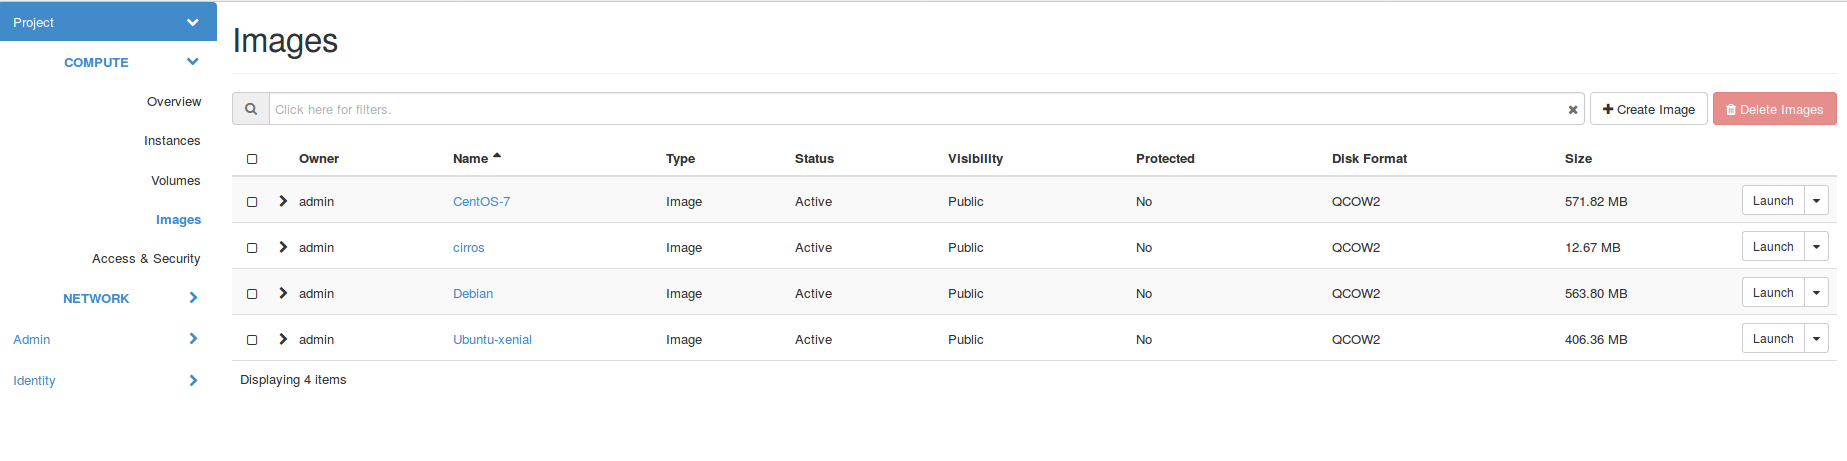
\includegraphics[width=6in]{./figures/createImage}
\caption{创建镜像}
\label{fig:createImage}
\end{figure}

\begin{figure}[!htb]
\centering
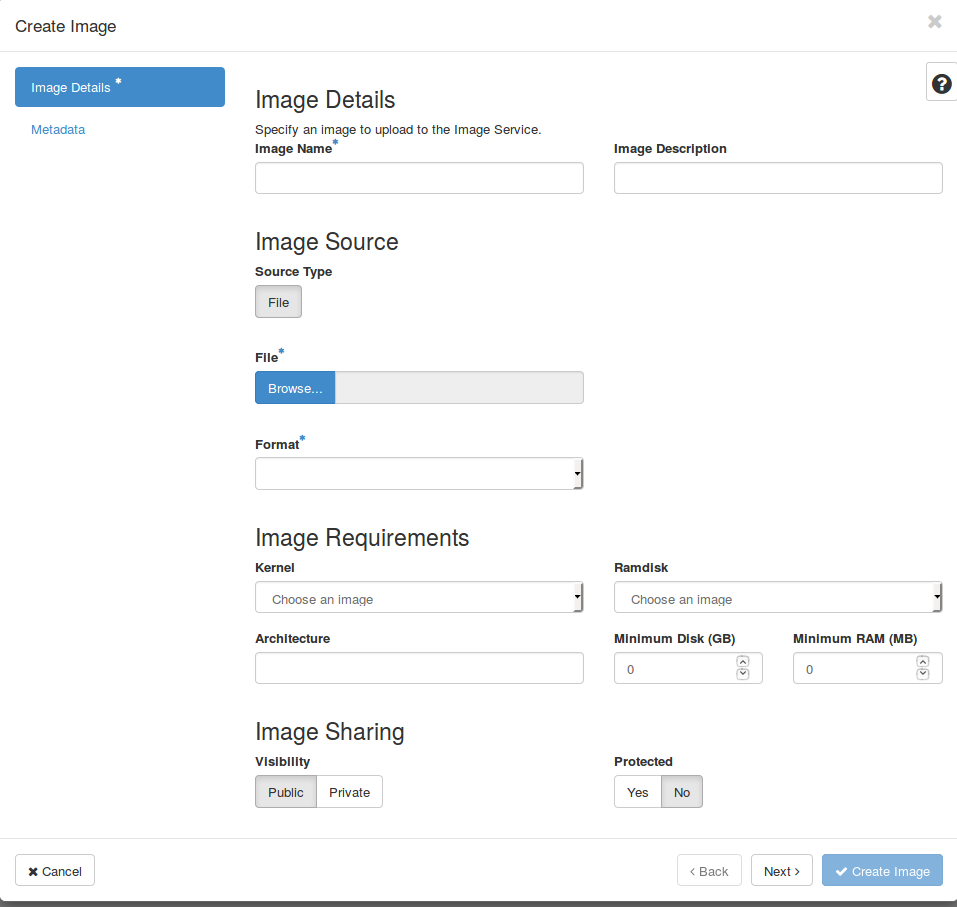
\includegraphics[width=6in]{./figures/createImageI}
\caption{创建镜像}
\label{fig:createImageI}
\end{figure}
\subsection{虚拟机管理}
用户有2种方式登陆虚拟机,ssh和console。下面主要介绍ssh登陆方式。
\subsubsection{虚拟机启动}
在写作平台管理界面,点击``\textbf{Project}''->``\textbf{Compute}''->``\textbf{Images}'',在拟启动镜像栏最右侧,点击``\textbf{Launch}'',在如图\ref{fig:launchInstanceI}弹出窗口中输入虚拟机名以及拟启动虚拟机数量。其中在如图\ref{fig:launchInstanceII},选择拟启动虚拟机的配置,如CPU数量、内存大小以及硬盘大小等;在如图\ref{fig:launchInstanceIII},选择虚拟机网络提供商;点击``\textbf{Key Pair}'',在如图\ref{fig:launchInstanceKey}弹出窗口中设置SSH登陆密钥。用户可以直接选择已有密钥如图\ref{fig:launchInstanceKey}下半窗口所示,也可以点击``\textbf{+Create Key Pair}''创建新密钥对。将创建的密钥\textbf{*.pem}文件保存至本地用于后续ssh登陆该虚拟机。
\begin{figure}[!htb]
\centering
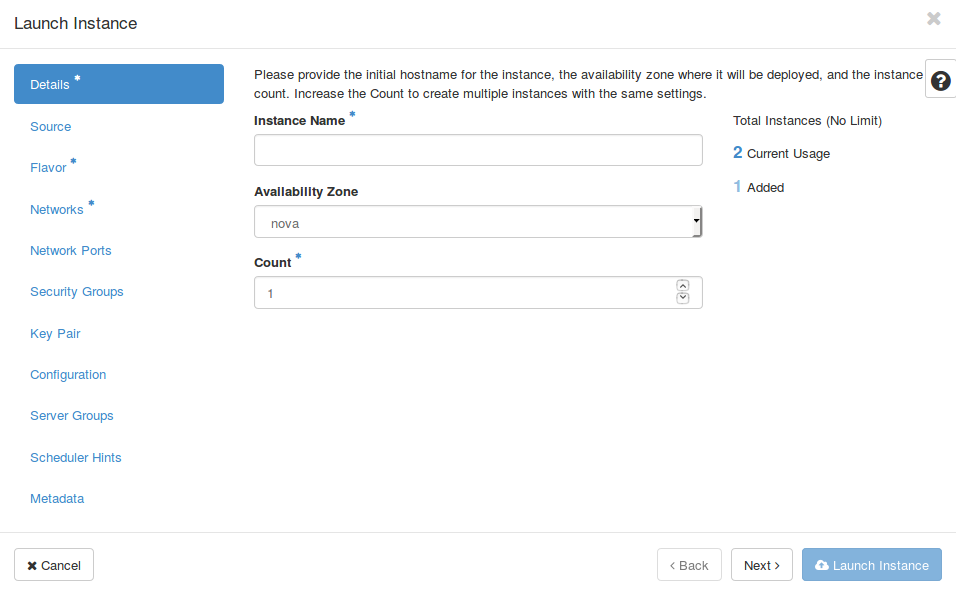
\includegraphics[width=6in]{./figures/launchInstanceI}
\caption{启动虚拟机}
\label{fig:launchInstanceI}
\end{figure}

\begin{figure}[!htb]
\centering
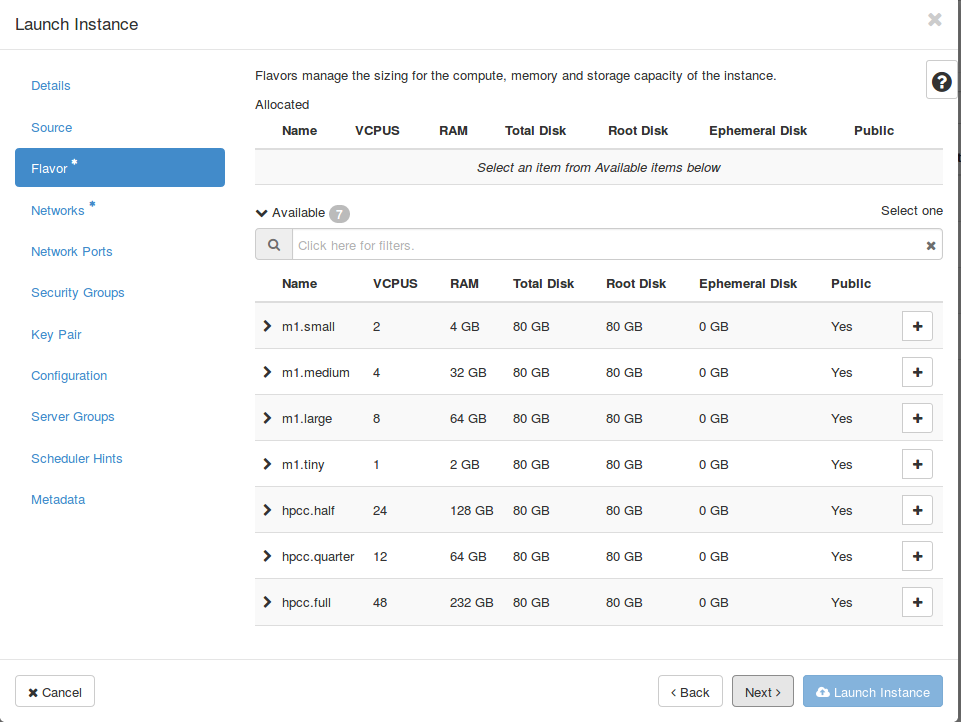
\includegraphics[width=6in]{./figures/launchInstanceII}
\caption{启动虚拟机}
\label{fig:launchInstanceII}
\end{figure}
\begin{figure}[!htb]
\centering
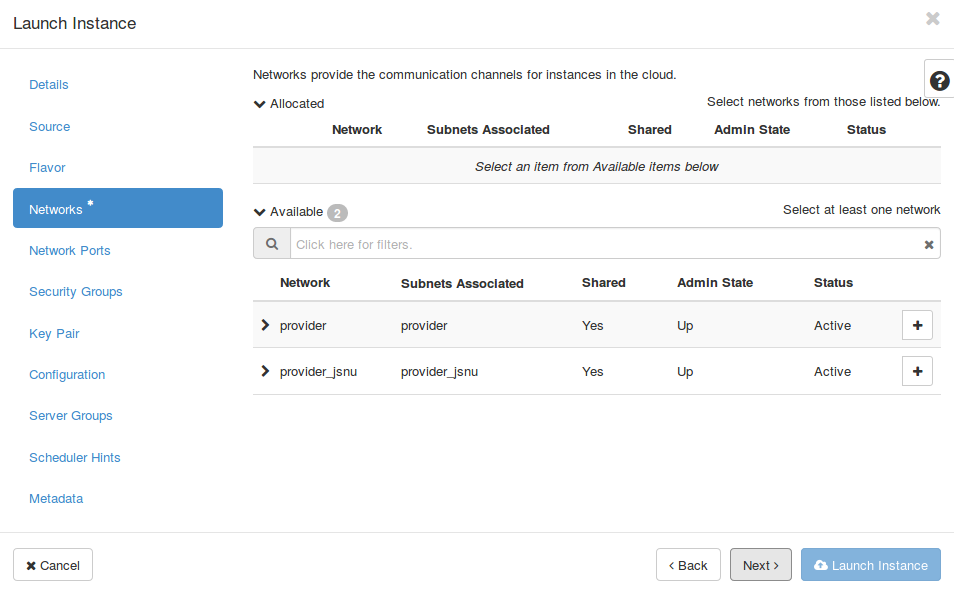
\includegraphics[width=6in]{./figures/launchInstanceIII}
\caption{启动虚拟机}
\label{fig:launchInstanceIII}
\end{figure}
\begin{figure}[!htb]
\centering
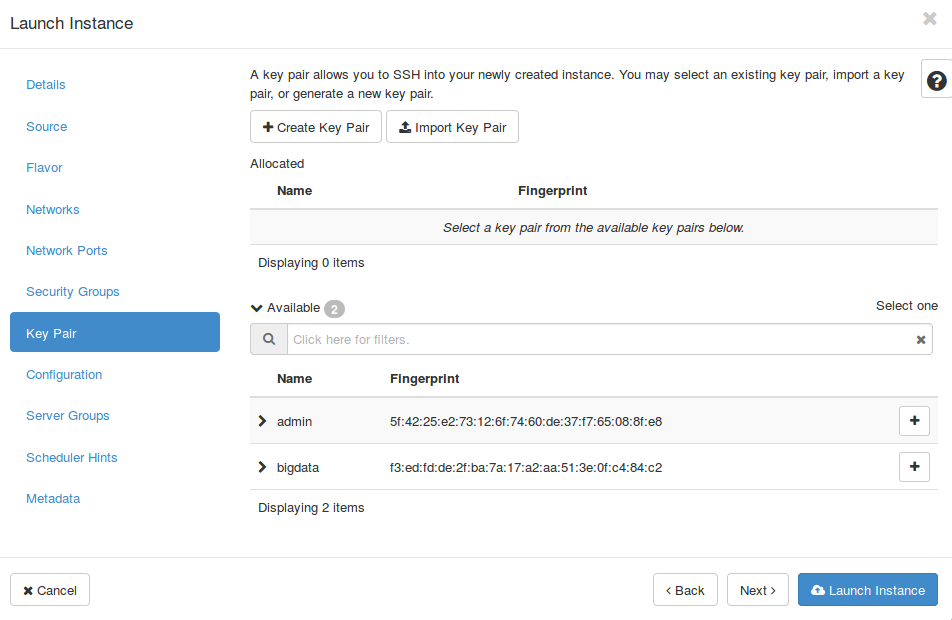
\includegraphics[width=6in]{./figures/launchInstanceKey}
\caption{启动虚拟机}
\label{fig:launchInstanceKey}
\end{figure}
用户也可以通过如图\ref{fig:launchInstanceConfig}为虚拟机添加运行脚本,例如修改用户密码、修改登陆配置等。最后点击``\textbf{Launch Instance}''完成虚拟机启动。
\begin{figure}[!htb]
\centering
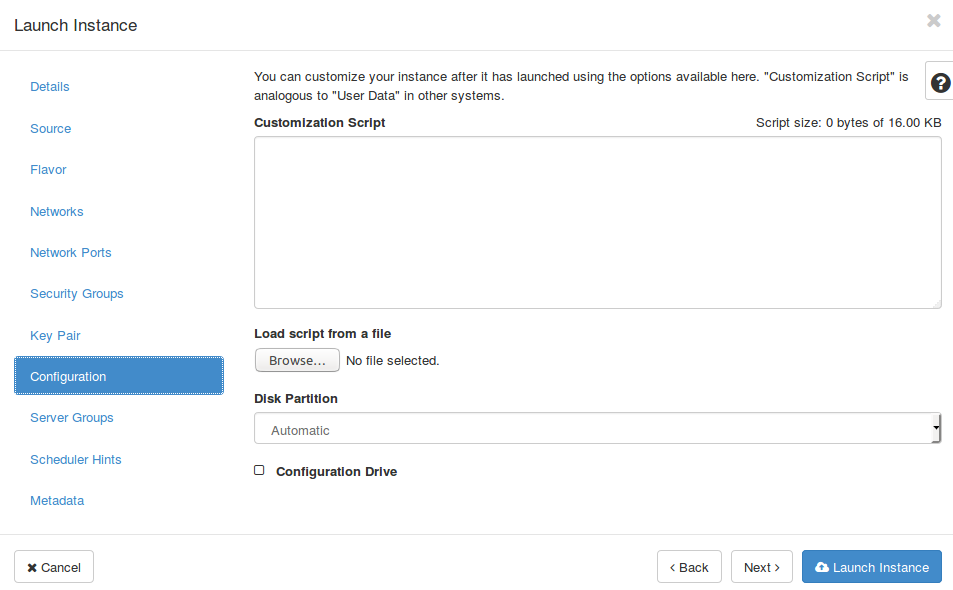
\includegraphics[width=6in]{./figures/launchInstanceConfig}
\caption{设置虚拟机运行脚本}
\label{fig:launchInstanceConfig}
\end{figure}

\subsubsection{虚拟机登陆}
虚拟机启动完毕,在``\textbf{Project}''->``\textbf{Compute}''->``\textbf{Instance}''能够看到该虚拟机ip地址、配置等信息如图\ref{fig:viewInstance}所示。
\begin{figure}[!htb]
\centering
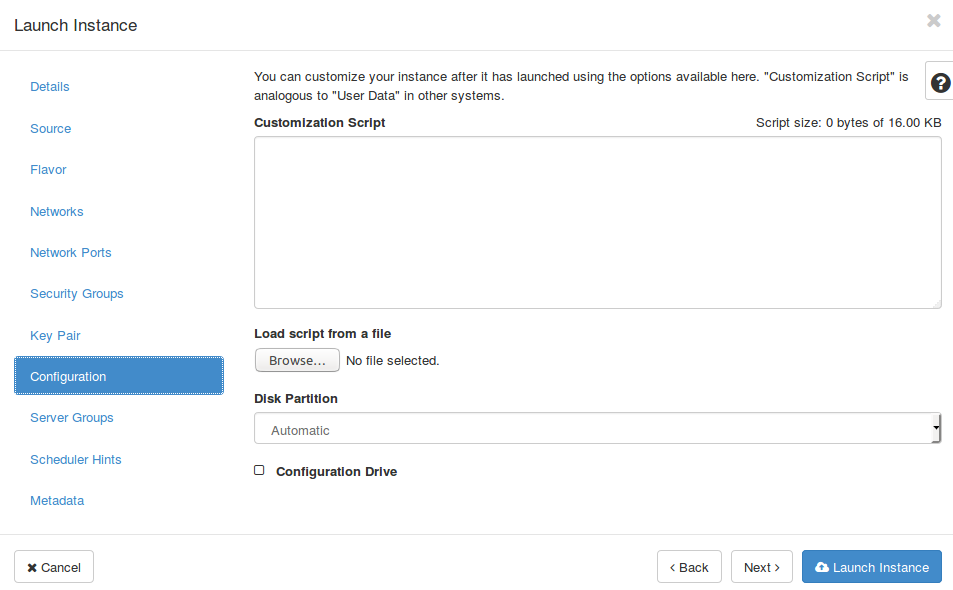
\includegraphics[width=6in]{./figures/launchInstanceConfig}
\caption{设置虚拟机运行脚本}
\label{fig:launchInstanceConfig}
\end{figure}
用户可以通过SSH登陆该虚拟机,具体指令结构如下:
ssh -i *.pem name@ip
其中,*.pem为在启动虚拟机时创建的密钥,注意此处必须给出该密钥的完整地址,同时该密钥文件的权限必须是600,即只有主用户有读写权限,组用户跟其他用户没有任何权限;name是该虚拟机中用户名,不同镜像通常拥有不同用户名,表\ref{tab:userName}给出常见镜像系统用户名。
\begin{table}[!htb]
\centering
\caption{常见镜像默认登陆用户名}
\label{tab:userName}
\begin{tabular}{|c|c|} \hline
 镜像 &登陆名\\ \hline
 ubuntu& ubuntu\\ \hline
 debian& debian\\ \hline
 centos& centos\\ \hline
\end{tabular}
\end{table}
\end{document}
